
\chapter{Results} 
  The main results of this thesis are give here:
    the cross section for coherent \JPsi production, the incoherent \JPsi cross
    section, the cross section for muon pairs from photon-photon interactions,
    the ratio between break up mode yields, and the rapidity correlations 
    between dimuon candidates and neutrons in the ZDC.

  \section{Coherent cross section}
  The coherent cross section in calculated from the following equation:
  \begin{equation}
    \frac{d\sigma^{J/\psi}_{co}}{dy}  = \frac{N_{cor} f_{co}  }
    { \Delta y~\mathcal{L}_{int} \varepsilon_{ZDC} \varepsilon_{p_{T}} 
      BR_{\mu^{+}\mu^{-}}}
    \label{eq:expXSecCo}
   \end{equation}
   where $N_{cor}$ is corrected dimuon yield, $f_{co}$ is the 
     fraction of events that come from the coherent process, 
     $BR_{\mu^{+}\mu^{-}}$ is the branching ratio for \JPsi to $\mu^{+}\mu^{-}$, 
     $\varepsilon_{ZDC}$ is the efficiency for triggering the ZDC, 
     $\varepsilon_{p_{T}}$ is the efficiency for the 0.15 GeV cut in $p_{T}$, 
     $\mathcal{L}_{int}$ is the integrated luminosity, and $\Delta y$ is the 
     width the rapidity interval.

  The raw yield of dimuon candidates was measured after applying the cuts 
    described in Section~\ref{sec:DataSetEvSel}.
  \begin{figure}[!Hhtb]
    \centering
    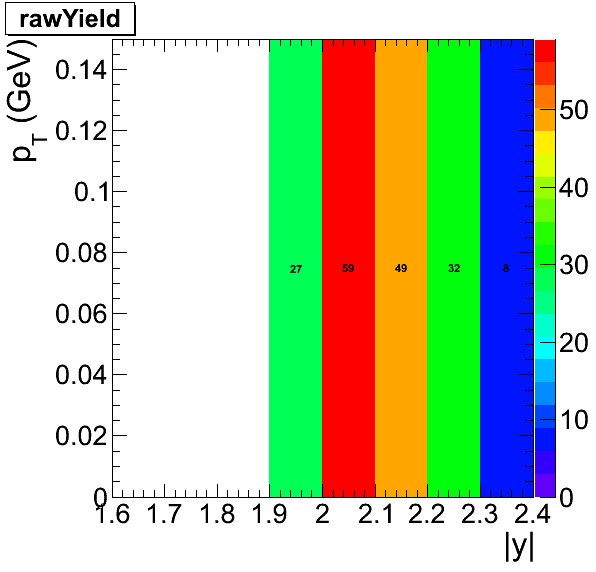
\includegraphics[width=0.6\textwidth]{rawYield}
    \caption{Raw yield for the Coherent cross section measurement.}
    \label{fig:rawYieldCo}
  \end{figure}
  $N_{cor}$ was calculated by dividing the raw yields from 
    Fig.~\ref{fig:rawYieldCo} by the acceptance and efficiency factor from 
    Fig.~\ref{fig:avAccEff}, which combines $A$ and 
    $\varepsilon^{dimuon}_{trigger}$ as described in Section.~\ref{sec:effDet}.
  The corrected yields, $N_{cor}$, are shown in Fig.~\ref{fig:corYieldCo}.
  \begin{figure}[!Hhtb]
    \centering
    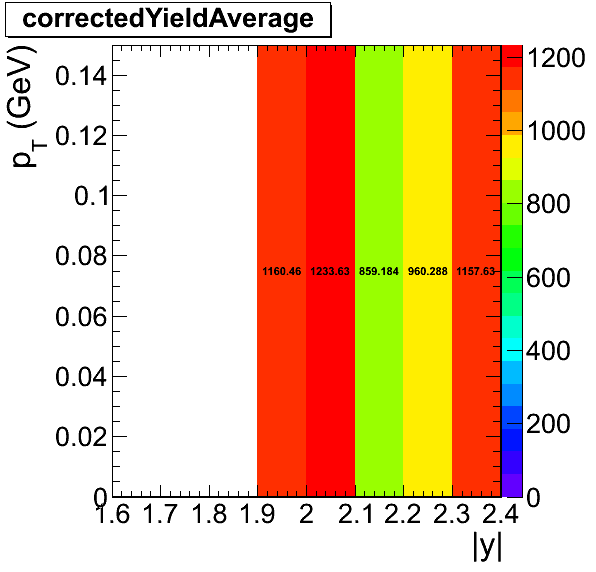
\includegraphics[width=0.6\textwidth]{correctedYieldAverage}
    \caption{Corrected yields for the coherent p$_{T}$ region.}
    \label{fig:corYieldCo}
  \end{figure}
  For the coherent cross section measurement, $N_{cor}$ is taken from the 
    region 2.0 < $|y|$ < 2.2 and $p_{T}$ < 0.15 GeV to avoid the edges of the
    detectors acceptance, bin migration in the calculation of $A$, and overlap
    between the coherent and incoherent process.
  From this procedure\DIFaddbegin \DIFadd{, }\DIFaddend the $N_{cor}$ was measured to be 1903.

  To measure $f_{co}$, the simultaneous fit shown in 
    Fig.~\ref{fig:simFitMassPtGauss} was used.
  The normalizations for each of the three components to the signal are fixed 
  by the fit as described in Section~\ref{sec:sigEx}.
  The normalized coherent template is integrated up to 0.15 GeV in $p_{T}$ and
    divided by the integral of the data $p_{T}$ spectrum up to 0.15 GeV.
  The statistical error taken from the fit, $f_{co}$ = 0.60 $\pm$ 0.11.

  The two efficiency terms, $\varepsilon_{ZDC}$ and $\varepsilon_{p_{T}}$, were
    measured from data and MC respectively.
  As described in Section~\ref{sec:breakUpDet}, $\varepsilon_{ZDC}$ was 
    measured in the from the ZDC triggered data set by dividing the number of 
    events both fire the ZDC trigger and pass the one neutron threshold.
  $\varepsilon_{ZDC}$ was measured to be 0.96 with a negligible statistical 
    error.
  The efficiency of the 0.15 GeV $p_{T}$ cut was estimated from MC by dividing 
    the number of events that are lost by applying the $p_{T}$ cut after all
    other cuts are applied. 
  From this method $\varepsilon_{p_{T}}$ = 0.95.

  The remaining two terms, $\mathcal{L}_{int}$ and $BR_{\mu^{+}\mu^{-}}$, 
    depend on Ref.~\cite{cmsLumi} and Ref.~\cite{pdg}.
  Ref.~\cite{cmsLumi} describes the method of using activity in HF to measure 
    the luminosity. 
  From this method, $\mathcal{L}_{int}$ was measured to be 143.3$\mu b^{-1}\pm$7.2.
  $BR_{\mu^{+}\mu^{-}}$ from Ref.~\cite{pdg} is 0.0593 $\pm$ 0.0006.
  From Equation~\ref{eq:expXSecCo}, $\frac{d\sigma^{J/\psi}_{co}}{dy}$ = 368 $mb$.

  \section{Incoherent cross section}
  \section{Break up ratios}
    In Table~\ref{tab:r2} the ratio between raw yields for different break up 
      modes are shown.
    \begin{figure}[!Hhtb]
      \centering
      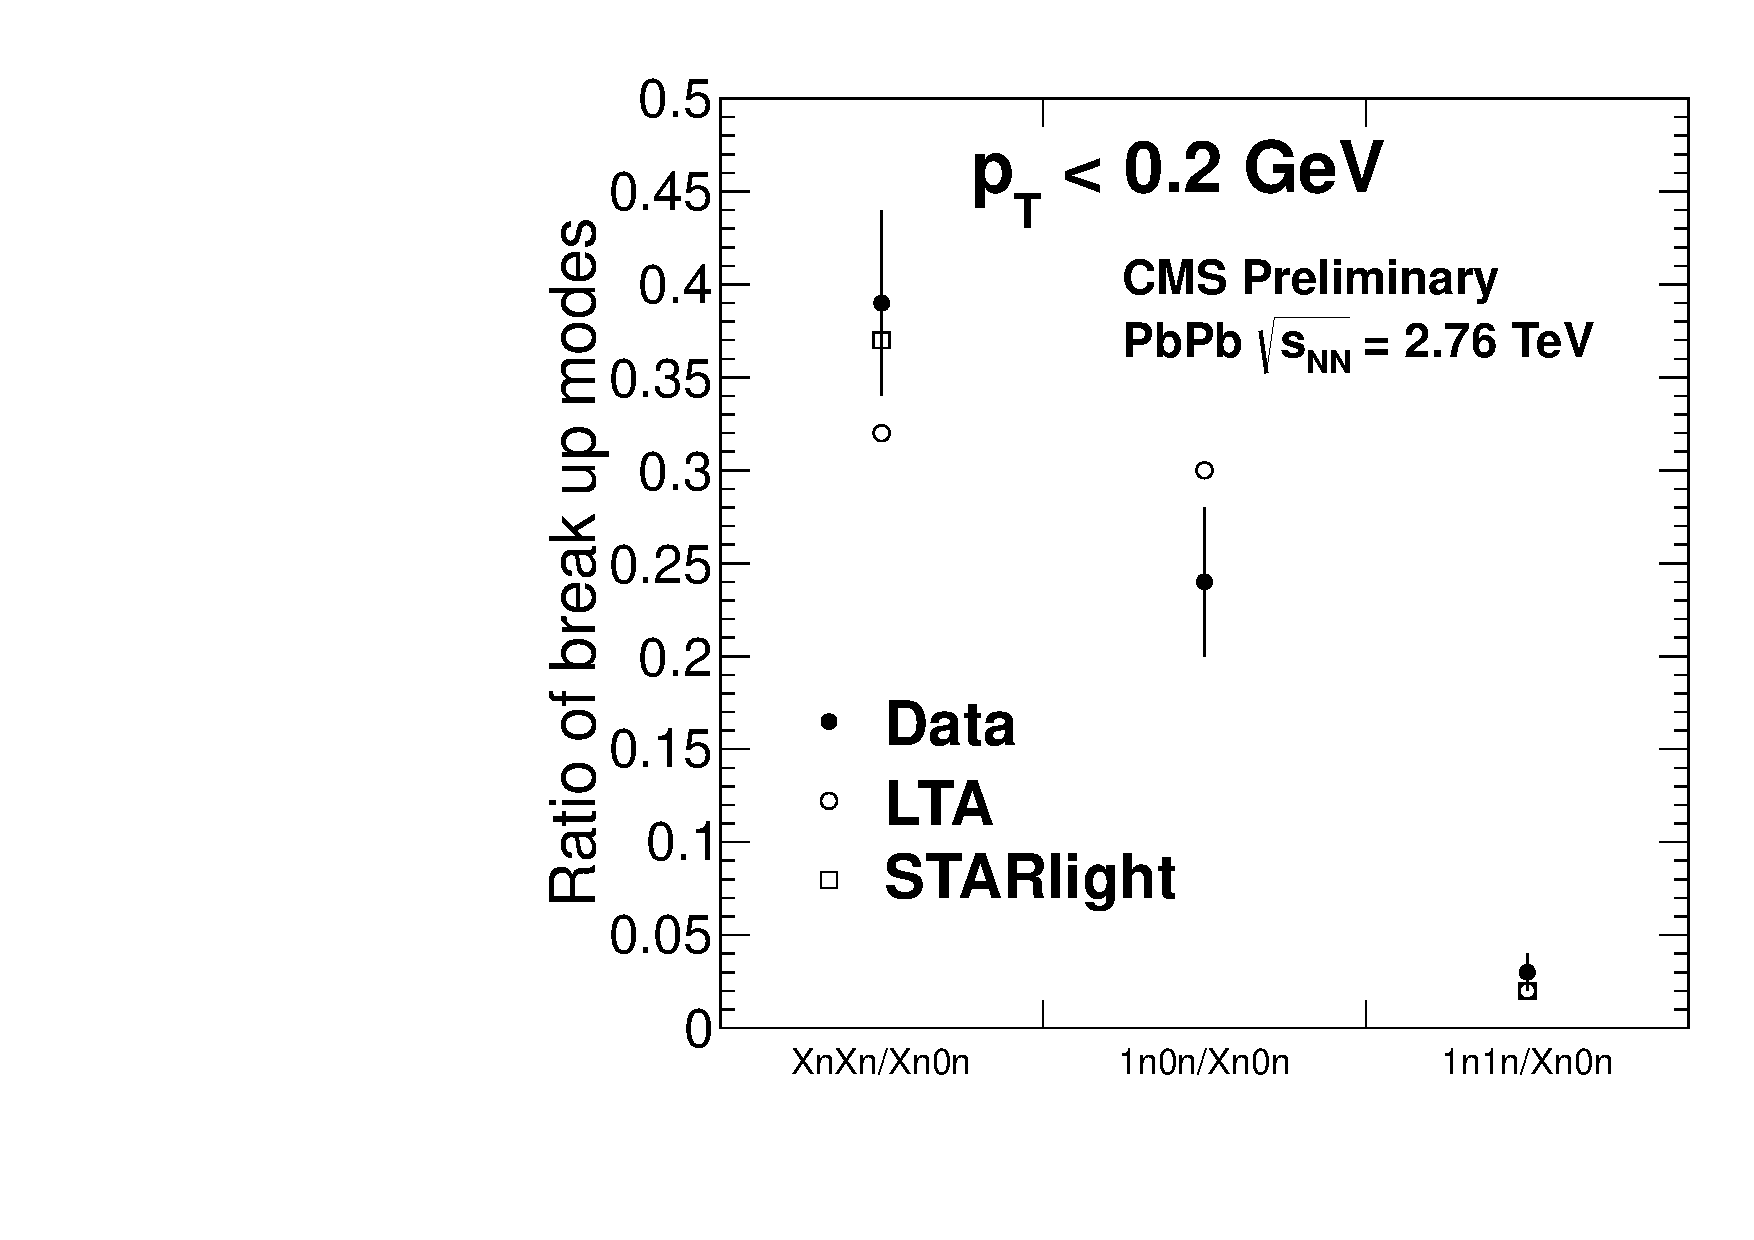
\includegraphics[width=.6\textwidth]{coherentBreakup}
      \caption{Ratio between J/$\psi$ yeilds XnXn and 1n0n break-up modes 
        compared the Xn0n break-up mode for J/$\psi$ with $p_{T}$ below 150 
        MeV.}
      \label{fig:coherentBreakUp}
    \end{figure}

    Fig.~\ref{fig:coherentBreakUp} and Fig.~\ref{fig:incoherentBreakUp} compare
      the raw break up ratios two STARlight and LTA predictions. 
    \DIFdelbegin %DIFDELCMD < 

%DIFDELCMD <     %%%
\DIFdelend \begin{figure}[!Hhtb]
      \centering
      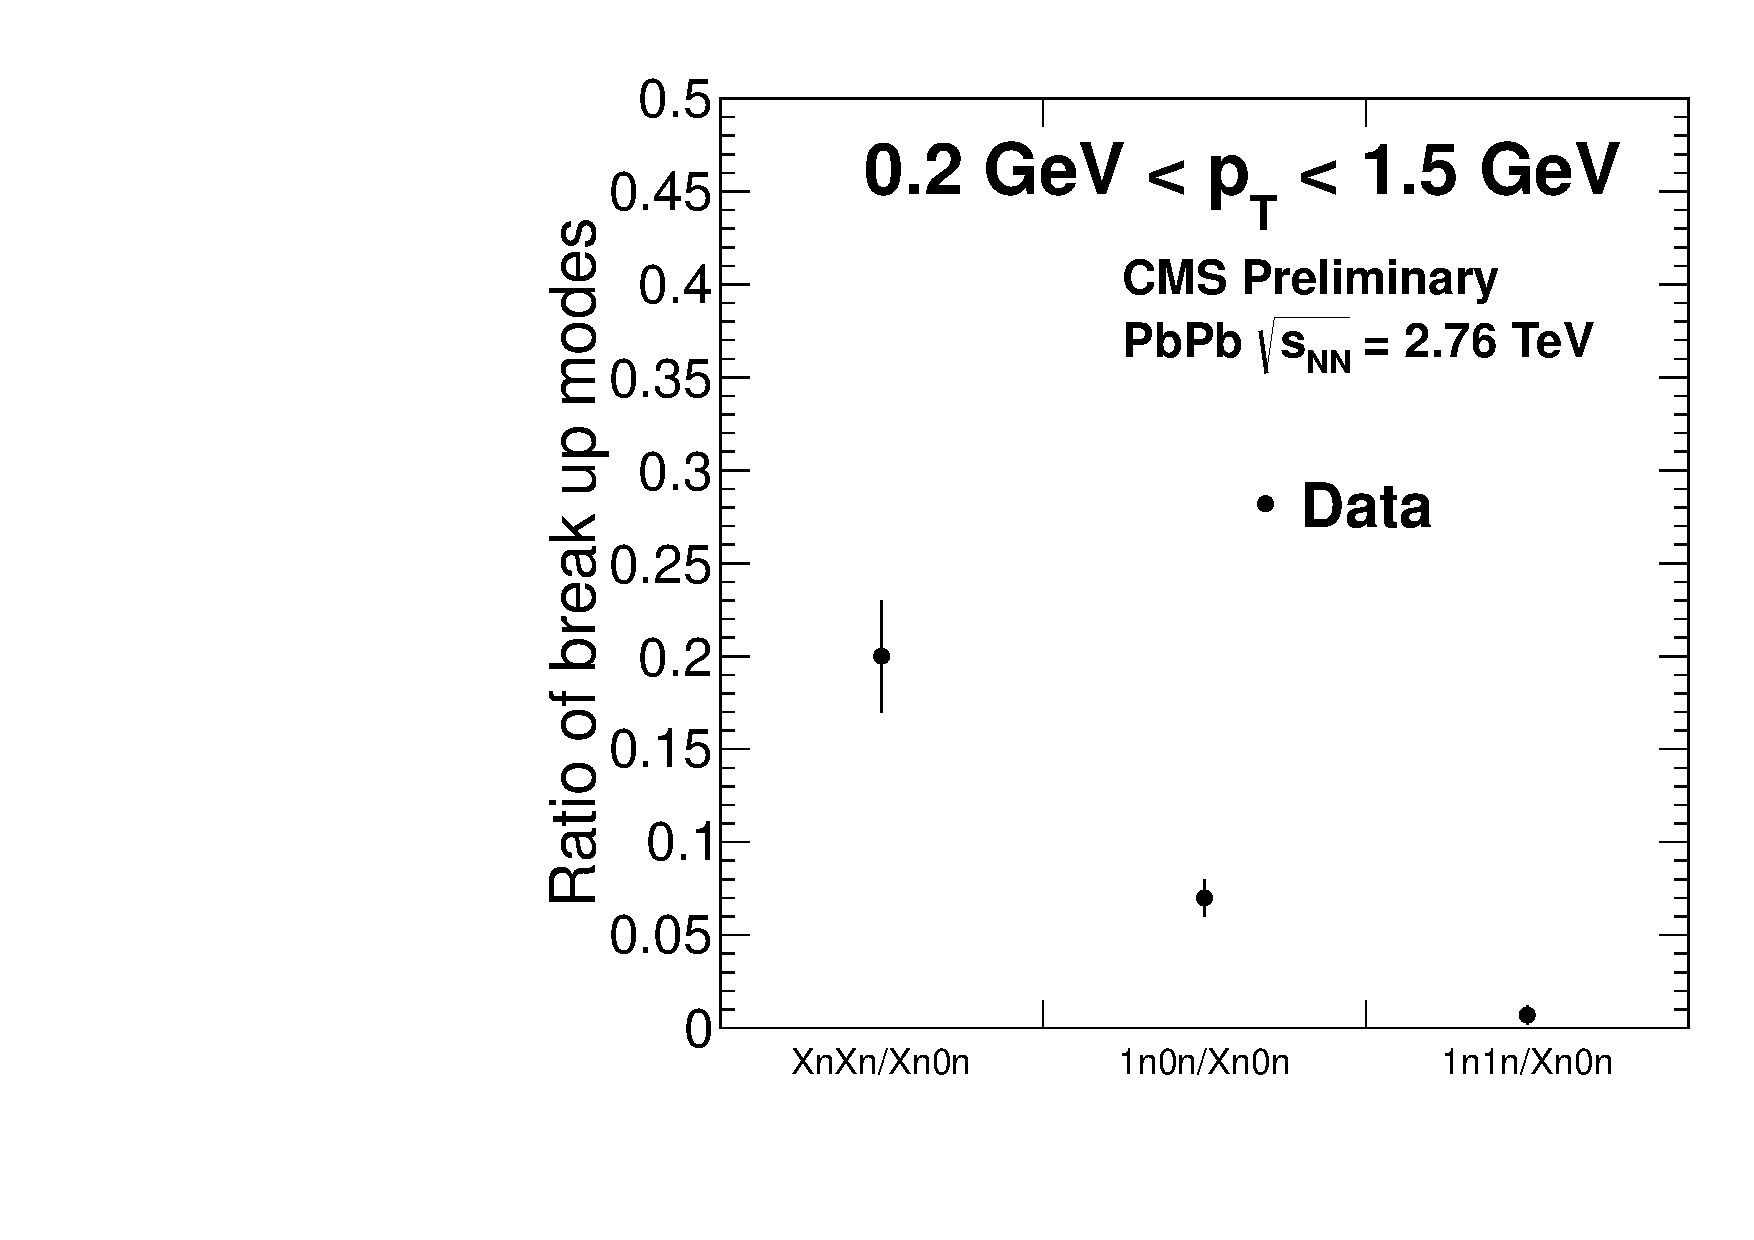
\includegraphics[width=.6\textwidth]{incoherentBreakup}
      \caption{Ratio between J/$\psi$ yeilds XnXn and 1n0n break-up modes 
        compared the Xn0n break-up mode for J/$\psi$ with 0.2 $< p_{T} <$ 
        1.5 GeV.}
      \label{fig:incoherentBreakUp}
    \end{figure}

    \DIFdelbegin \DIFdel{In Table~\ref{tab:r3} the ratio between break up modes are shown for 
      different theories and processes.
}%DIFDELCMD < 

%DIFDELCMD <     \begin{table}[h]
%DIFDELCMD <       \begin{center}
%DIFDELCMD <         %%%
%DIFDELCMD < \caption{%
{%DIFAUXCMD
\DIFdel{Number of  J/$\psi$ integrated over $p_{T}$ and $y$ with statistical uncertainty.}}
        %DIFAUXCMD
%DIFDELCMD < \label{tab:r3}
%DIFDELCMD <         \begin{tabular}{|c|c|c|c|c|}
%DIFDELCMD <           \hline
%DIFDELCMD <           & %%%
\DIFdel{X$_{n}$X$_{n}$/X$_{n}$0$_{n}$ }%DIFDELCMD < & %%%
\DIFdel{1$_{n}$0$_{n}$/X$_{n}$0$_{n}$ }%DIFDELCMD < & %%%
\DIFdel{1$_{n}$1$_{n}$/X$_{n}$0$_{n}$  }%DIFDELCMD < \\ 
%DIFDELCMD <           \hline
%DIFDELCMD <           %%%
\DIFdel{STARlight coherent }%DIFDELCMD < &  %%%
\DIFdel{0.37}%DIFDELCMD < &%%%
\DIFdel{-}%DIFDELCMD < &%%%
\DIFdel{0.02}%DIFDELCMD < \\
%DIFDELCMD <           \hline
%DIFDELCMD <           %%%
\DIFdel{Zhalov coherent}%DIFDELCMD < & %%%
\DIFdel{0.32}%DIFDELCMD < &%%%
\DIFdel{0.30}%DIFDELCMD < &%%%
\DIFdel{0.02}%DIFDELCMD < \\
%DIFDELCMD <           \hline
%DIFDELCMD <           %%%
\DIFdel{STARlight incoherent }%DIFDELCMD < &  %%%
\DIFdel{0.37}%DIFDELCMD < &%%%
\DIFdel{-}%DIFDELCMD < &%%%
\DIFdel{0.007$\pm$0.02 }%DIFDELCMD < \\
%DIFDELCMD <           \hline
%DIFDELCMD <         \end{tabular}
%DIFDELCMD <       \end{center}
%DIFDELCMD <     \end{table}
%DIFDELCMD < 

%DIFDELCMD <   %%%
\section{\DIFdel{diMuon-neutron correlations}}
    %DIFAUXCMD
\addtocounter{section}{-1}%DIFAUXCMD
\DIFdel{The invariant mass distribution for different break-up modes is show for the coherent and incoherent J/$\psi$ on the Fig.~\ref{fig:r1} and Fig.~\ref{fig:r2} respectively. 
    }%DIFDELCMD < \begin{figure*}[!Hhtb]
%DIFDELCMD <       \begin{center}
%DIFDELCMD <         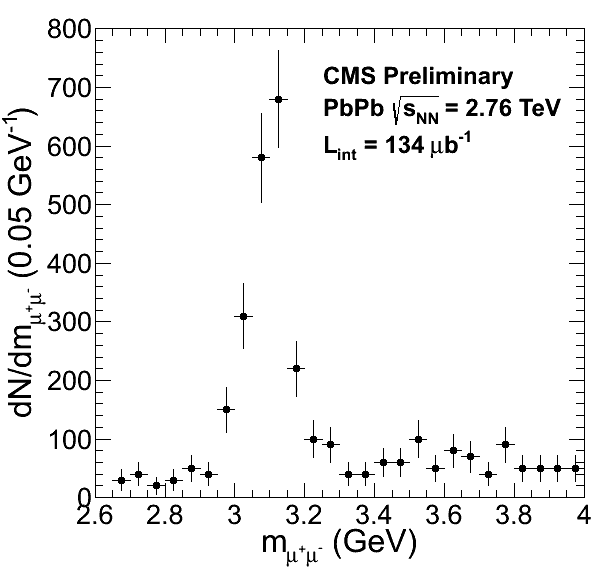
\includegraphics[angle=0,width=0.45\textwidth]{coherentJPsiMass.png}
%DIFDELCMD <         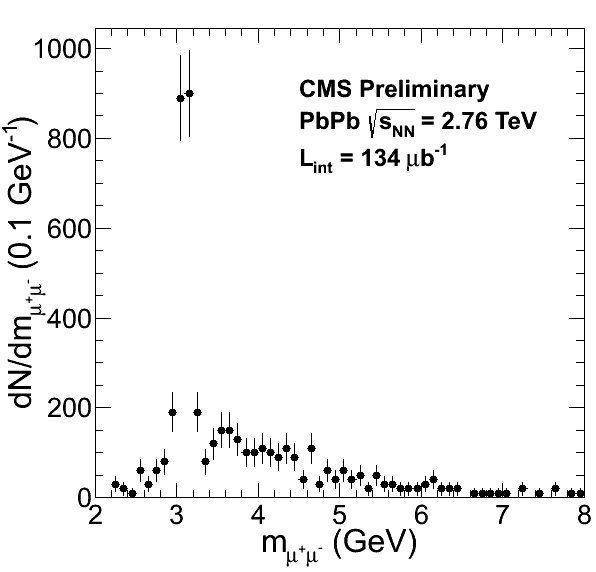
\includegraphics[angle=0,width=0.45\textwidth]{coherentMass.png}
%DIFDELCMD <         %%%
%DIFDELCMD < \caption{%
{%DIFAUXCMD
\DIFdel{
          \label{fig:r1}  
          Invariant mass spectrum of the opposite signs di-muons originating from the coherent J/$\psi$ for $X_{n}0_{n}$ breakup mode for two invariant mass regions.  
        }}
      %DIFAUXCMD
%DIFDELCMD < \end{center}
%DIFDELCMD <     \end{figure*}
%DIFDELCMD <     

%DIFDELCMD <     \begin{figure*}[!Hhtb]
%DIFDELCMD <       \begin{center}
%DIFDELCMD <         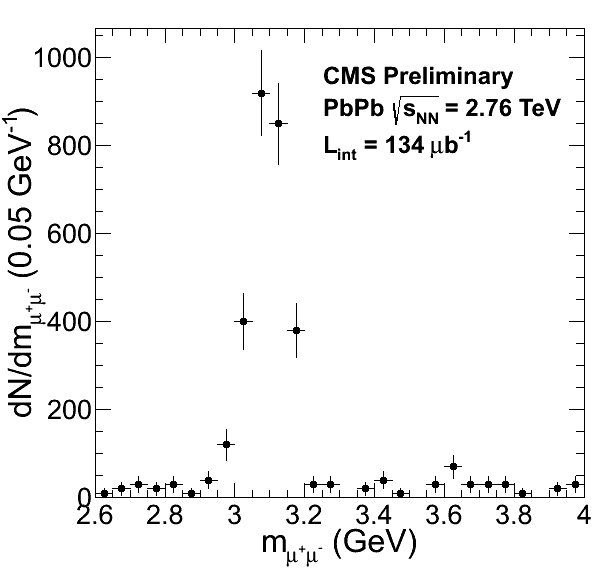
\includegraphics[angle=0,width=0.45\textwidth]{incoherentJPsiMassInCo.png}
%DIFDELCMD <         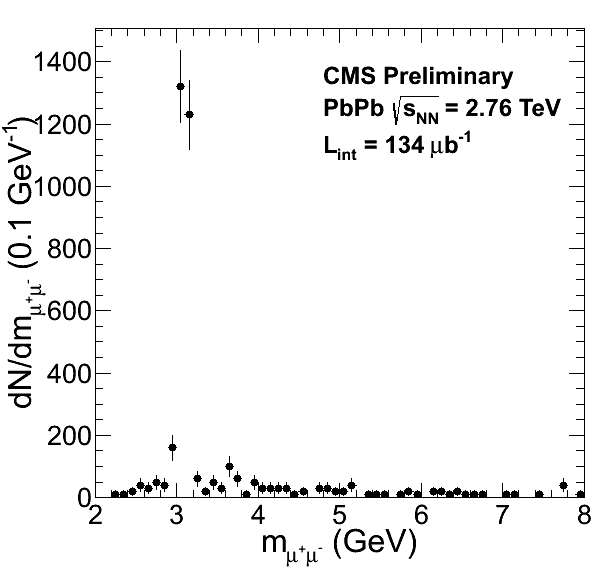
\includegraphics[angle=0,width=0.45\textwidth]{incoherentMassInCo.png}
%DIFDELCMD <         %%%
%DIFDELCMD < \caption{%
{%DIFAUXCMD
\DIFdel{
          Invariant mass spectrum of the opposite signs di-muons originating
          from the incoherent J/$\psi$  for $X_{n}0_{n}$ breakup mode for two 
          invariant mass regions.   
        }}
        %DIFAUXCMD
%DIFDELCMD < \label{fig:r2}  
%DIFDELCMD <       \end{center}
%DIFDELCMD <     \end{figure*}
%DIFDELCMD <     

%DIFDELCMD <     %%%
\DIFdelend The number of the coherent and incoherent J/$\psi$ for each break-up mode are
      given in the Tab.~\ref{tab:r1}. 
    The ratios between the modes X$_{n}$X$_{n}$, 1$_{n}$0$_{n}$, 1$_{n}$1$_{n}$ and
      the mode  X$_{n}$0$_{n}$ are given in the table Tab.~\ref{tab:r2}. 
    Some of the  ratios can be obtained from  {\sc starlight} and from the Zhalov 
      and thus are given in Tab.~\ref{tab:r3}.
    \DIFdelbegin %DIFDELCMD < 

%DIFDELCMD <     %%%
\DIFdelend \begin{table}[h]
      \begin{center}
      \DIFdelbeginFL %DIFDELCMD < \caption{%
{%DIFAUXCMD
\DIFdelFL{Number of coherent J/$\psi$ integrated over $p_{T}$ and $y$ with statistical uncertainty.}}
    %DIFAUXCMD
%DIFDELCMD < \label{tab:r1}
%DIFDELCMD <     %%%
\DIFdelendFL \begin{tabular}{|c|c|c|c|c|c|}
        \hline
         &  X$_{n}$0$_{n}$& X$_{n}$X$_{n}$ & 1$_{n}$0$_{n}$ & 1$_{n}$1$_{n}$  \\ \hline
        coherent J/$\psi$ &  242$\pm$16&94$\pm$10&58$\pm$8&8$\pm$3\\ \hline
        incoherent J/$\psi$ & 291$\pm$17&57$\pm$8&19$\pm$4&2$\pm$1\\ \hline
      \end{tabular}
      \DIFaddbeginFL \caption{\label{tab:r1} \DIFaddFL{Number of coherent J/$\psi$ integrated over $p_{T}$ and $y$ 
        with statistical uncertainty.}}
      \DIFaddendFL \end{center}
    \DIFdelbeginFL %DIFDELCMD < 

%DIFDELCMD <     %%%
\DIFdelendFL \end{table}

    \begin{table}[h]
      \begin{center}
        \DIFdelbeginFL %DIFDELCMD < \caption{%
{%DIFAUXCMD
\DIFdelFL{Number of coherent J/$\psi$ integrated over $p_{T}$ and $y$ 
          with statistical uncertainty.}}
        %DIFAUXCMD
%DIFDELCMD < \label{tab:r2}
%DIFDELCMD <         %%%
\DIFdelendFL \begin{tabular}{|c|c|c|c|c|}
          \hline
          & X$_{n}$X$_{n}$/X$_{n}$0$_{n}$ & 1$_{n}$0$_{n}$/X$_{n}$0$_{n}$ & 1$_{n}$1$_{n}$/X$_{n}$0$_{n}$  \\ \hline
          coherent J/$\psi$ &  0.39$\pm$0.05&0.24$\pm$0.04&0.03$\pm$0.01\\ \hline
          incoherent J/$\psi$ &  0.20$\pm$0.03&0.07$\pm$0.02&0.007$\pm$0.005 \\ \hline
        \end{tabular}
      \DIFaddbeginFL \caption{\label{tab:r2} \DIFaddFL{Number of coherent J/$\psi$ integrated over $p_{T}$ and $y$ 
        with statistical uncertainty.}}
      \DIFaddendFL \end{center}
    \end{table}

    \DIFdelbegin \DIFdel{For statistical reason, further studies concentrate only on the break-up mode 
      }\DIFdelend \DIFaddbegin \DIFadd{In Table~\ref{tab:r3} the ratio between break up modes are shown for 
      different theories and processes.
    }\begin{table}[h]
      \begin{center}
        \begin{tabular}{|c|c|c|c|c|}
          \hline
          & \DIFaddendFL X$_{n}$\DIFaddbeginFL \DIFaddFL{X$_{n}$/X$_{n}$}\DIFaddendFL 0$_{n}$ \DIFdelbeginFL \DIFdelFL{. }%DIFDELCMD < \\
%DIFDELCMD <     %%%
\DIFdelFL{Figure~\ref{fig:r3} shows the transverse momentum distribution of the J}\DIFdelendFL \DIFaddbeginFL & \DIFaddFL{1$_{n}$0$_{n}$}\DIFaddendFL /\DIFdelbeginFL \DIFdelFL{$\psi$ 
      (coherent and incoherent) in the case when J}\DIFdelendFL \DIFaddbeginFL \DIFaddFL{X$_{n}$0$_{n}$ }& \DIFaddFL{1$_{n}$1$_{n}$}\DIFaddendFL /\DIFdelbeginFL \DIFdelFL{$\psi$ and neutron have the same
      or opposite rapidity direction.
          The ratio between the J/$\psi$ and neutronthat have the opposite direction and
      the J/$\psi$ and neutron that have the same direction i shown on 
      Fig.
          ~\ref{fig:r4}. 
      The red curve gives the 
        pure theory calculations, the black one gives the theory 
      results that are injected to }\DIFdelendFL \DIFaddbeginFL \DIFaddFL{X$_{n}$0$_{n}$  }\\ \hline
          \DIFaddFL{STARlight coherent }&  \DIFaddFL{0.37}&\DIFaddFL{-}&\DIFaddFL{0.02}\\ \hline
          \DIFaddFL{Zhalov coherent}& \DIFaddFL{0.32}&\DIFaddFL{0.30}&\DIFaddFL{0.02}\\ \hline
          \DIFaddFL{STARlight incoherent }&  \DIFaddFL{0.37}&\DIFaddFL{-}&\DIFaddFL{0.007$\pm$0.02 }\\ \hline
        \end{tabular}
        \caption{\label{tab:r3} \DIFaddFL{Number of  J/$\psi$ integrated over $p_{T}$ and $y$ with 
          statistical uncertainty.}}
      \end{center}
    \end{table}

  \section{\DIFadd{diMuon-neutron correlations}}
    \DIFadd{In this section the correlation between the rapidity of the $\mu^{+}\mu^{-}$ 
      and of the neutron is studied. The following samples are studied: 
    }\begin{itemize}
      \item \DIFadd{$\gamma + A$ collisions in which two cases are considered
      }\begin{itemize}
        \item \DIFadd{elastic coherent interaction: here photon interacts with entier
          nucleus coherently and produce }\JPsi\DIFadd{. 
          Another photon is needed to cause the breakup and neutron emission. 
          Those two photons are uncorrelated and thus we don't expect to 
            observe the correlation between the rapidity of the neutron and the
            rapidity of the }\JPsi\DIFadd{.
          In the data sample this corresponds to the low-}\pt \JPsi 
            \DIFadd{(}\pt\DIFadd{$<$0.15~GeV). 
        }\item \DIFadd{inelastic incoherent interaction: here a single high }\pt \DIFadd{photoni
          interacting with nucleus produce the }\JPsi \DIFadd{and neutron. 
          The correlation between the rapidity of the neutron and the rapidity
            of the }\JPsi \DIFadd{is expected.
          In the data sample this corresponds to the high-}\pt \JPsi 
            \DIFadd{(0.15$<$}\pt\DIFadd{$<$1.05). 
      }\end{itemize}
      \item \DIFadd{$\gamma \gamma$ collisions: two photons collide and produce the 
        $\mu^{+}\mu^{-}$  and the third photon is needed to excite one of
          the nucleons and produce neutron. 
        Thus we don't expect to see the correlation between the rapidity of the
          neutron and the rapidity of }\DIFaddend the \DIFdelbegin \DIFdel{detector simulation and thus taking into 
      account experimental bias. 
     }\DIFdelend \DIFaddbegin \DIFadd{$\mu^{+}\mu^{-}$. 
        In the data sample this corresponds to the $\mu^{+}\mu^{-}$ with the
          invariant mass between 4 and 8~GeV. 
    }\end{itemize}
\DIFaddend 

    \DIFaddbegin \DIFadd{In order to study the correlation in rapidity between the neutron and
      dimuon direction we below four quantities and give they values in 
      Table~\ref{tab:corrneutronjpsi}.  
    }\begin{itemize}
      \item \DIFadd{$y^{-}_{\mu\mu} \wedge y_{n}^{-}$: number of $\mu^{+}\mu^{-}$ having
         $y<0$ and the neutron in ZDC$^{-}$ ($y<0$)
      }\item \DIFadd{$y^{-}_{\mu\mu} \wedge y_{n}^{+}$: number of $\mu^{+}\mu^{-}$ having
         $y<0$ and the neutron in ZDC$^{+}$ ($y>0$)
      }\item \DIFadd{$y^{+}_{\mu\mu} \wedge y_{n}^{+}$: number of $\mu^{+}\mu^{-}$ having
         $y>0$ and the neutron in ZDC$^{+}$ ($y>0$)
      }\item \DIFadd{$y^{+}_{\mu\mu} \wedge y_{n}^{-}$: number of $\mu^{+}\mu^{-}$ having
         $y>0$ and the neutron in ZDC$^{-}$ ($y<0$)
    }\end{itemize}

    \DIFadd{The ratio $R_{opp/same}$ is defined as: 
    }\begin{equation}\DIFadd{
      R_{opp/same} = \frac{y^{-}_{\mu\mu} \wedge y_{n}^{+} + y^{+}_{\mu\mu} 
        \wedge y_{n}^{-}}{y^{-}_{\mu\mu} \wedge y_{n}^{-} + y^{+}_{\mu\mu} 
        \wedge y_{n}^{+}}
    }\end{equation}

    \DIFadd{Ratios studied in this section are only sensitive to the difference between
      the ZDC$^{-}$ and ZDC$^{-}$.
    It is seen that the efficiency of both ZDCs in not exactly the same i.e.
      the efficiencies of ZDC$^{-}$ and ZDC$^{+}$ are respectively 
      $\varepsilon_{ZDC^{-}}$=0.98 and  $\varepsilon_{ZDC^{+}}$=0.94 and this 
      is taken in the account in the estimations. 
    The $R_{opp/same}$ radio corrected by the ZDCs efficiencies is also 
      included in Table~\ref{tab:corrneutronjpsi} and called 
      $R_{opp/same}^{\varepsilon_{ZDC}}$. 
    It is seen that the difference between corrected and uncorrected results is
      very small. 
    Other uncertainties cancel. 
    In this case cuts related to the acceptance and efficiencies corrections 
      are not necessary and thus they are released.
    }

    \DIFadd{Figure~\ref{fig:PtcorrandRation} gives }\pt \DIFadd{distributions of the }\JPsi 
      \DIFadd{when }\JPsi \DIFadd{and neutron have the opposite rapidity direction or when they 
      have the same rapidity direction for low-}\pt \DIFadd{and high-}\pt \JPsi\DIFadd{. 
    Also the Fig~\ref{fig:PtcorrandRation} gives the $R_{opp/same}$ for low-}\pt
      \DIFadd{and high-}\pt \JPsi\DIFadd{. 
    In is send from this plot that in the case of the low-}\pt \JPsi \DIFadd{this 
      $R_{opp/same}$ ratio is close to 1 and is decreasing when the }\pt \DIFadd{of
      }\JPsi \DIFadd{increases.
  }

    \DIFaddend \begin{figure*}[!Hhtb]
      \begin{center}
        \DIFdelbeginFL %DIFDELCMD < 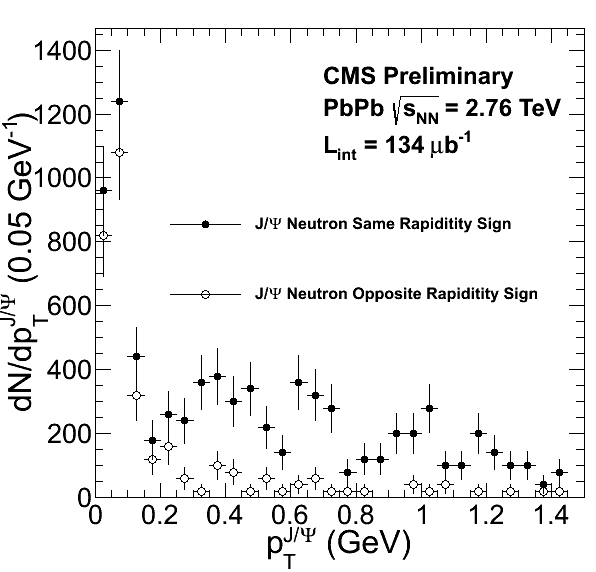
\includegraphics[angle=0,width=0.45\textwidth]{Pt.png}
%DIFDELCMD <             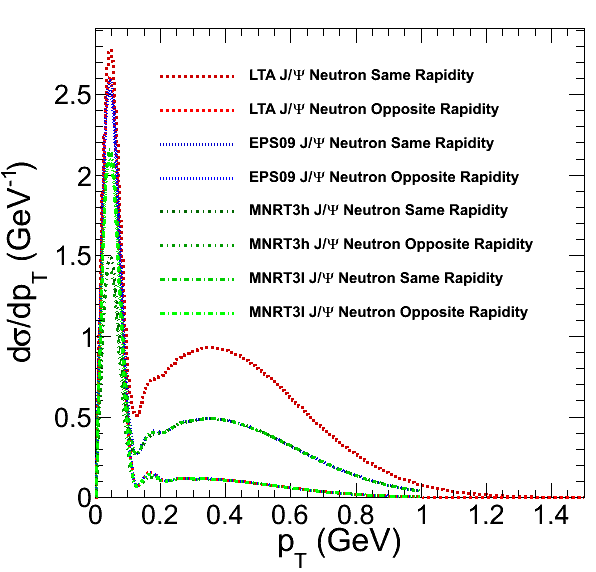
\includegraphics[angle=0,width=0.45\textwidth]{PtTheory.png}
%DIFDELCMD <                  %%%
%DIFDELCMD < \caption{%
{%DIFAUXCMD
\DIFdelFL{
        \label{fig:r3}  
         Transverse momentum distribution of the J/$\psi$ when J/$\psi$ and neutron have the same or opposite rapidity direction from data (left) and from theory (right). 
            }}
           %DIFAUXCMD
\DIFdelendFL \DIFaddbeginFL 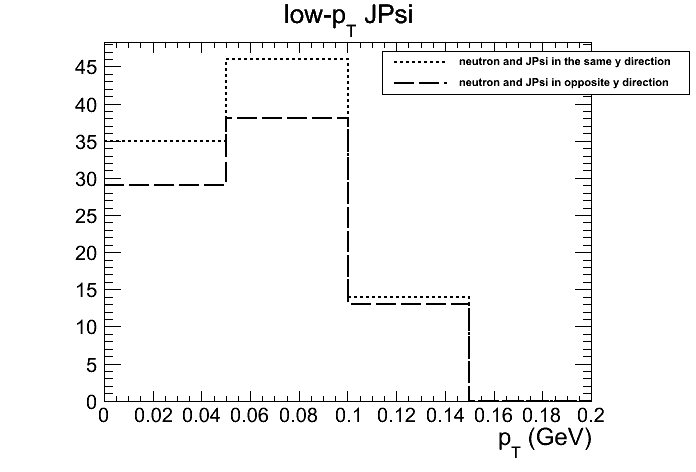
\includegraphics[angle=0,width=0.45\textwidth]{cohOppAndSameNeutronDir}
        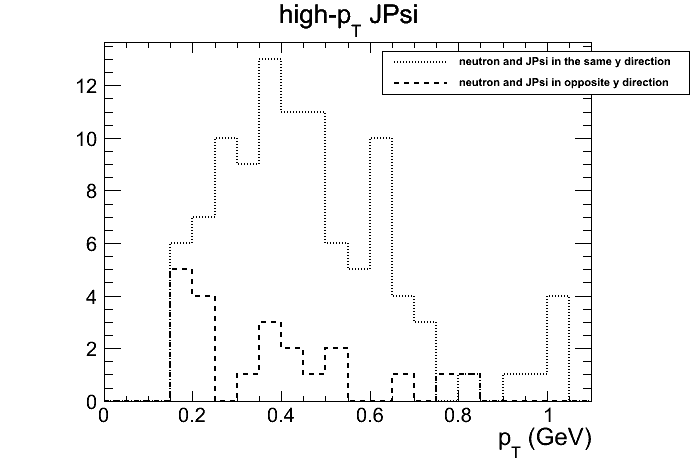
\includegraphics[angle=0,width=0.45\textwidth]{incohOppAndSameNeutronDir} \\
        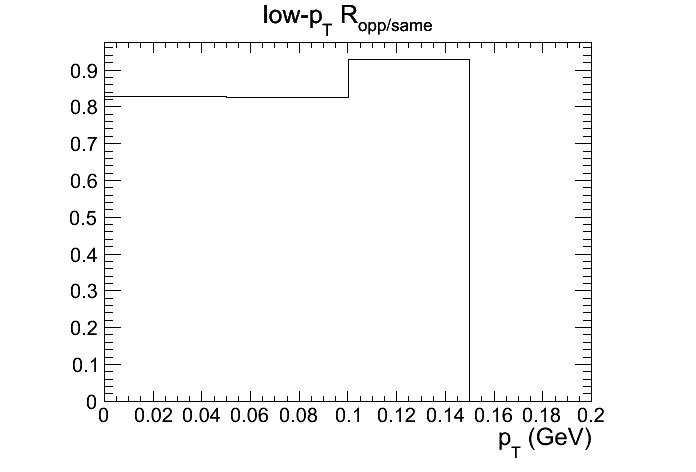
\includegraphics[angle=0,width=0.45\textwidth]{ratiocohOppAndSameNeutronDir}
        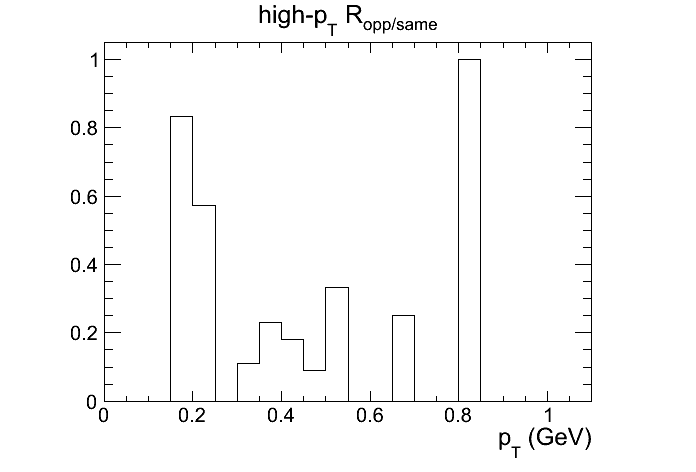
\includegraphics[angle=0,width=0.45\textwidth]{ratioincohOppAndSameNeutronDir}
      \caption{\DIFaddFL{ \label{fig:PtcorrandRation}  
        Transverse momentum distribution of the $J/\psi$ when  $J/\psi$ and 
          neutron have the opposite rapidity direction and the transverse 
          momentum distribution of the $J/\psi$ when  $J/\psi$ and neutron
          have the same rapidity direction for low-}\pt \DIFaddFL{(top left) and 
          high-}\pt \DIFaddFL{(top right) }\JPsi\DIFaddFL{. Bottom: Ratios $R_{opp/same}$ for 
          low-}\pt \DIFaddFL{( left) and high-}\pt \DIFaddFL{( right) }\JPsi\DIFaddFL{.}}
      \DIFaddendFL \end{center}
    \end{figure*}

    \DIFaddbegin \DIFadd{Compiled for }\pt\DIFadd{$<$1.05~GeV $R_{opp/same}$ ratio between the }\pt 
      \DIFadd{distribution of the }\JPsi \DIFadd{having neutron emitted in the opposite 
      direction and  the }\JPsi \DIFadd{having the neutron emitted in the same
      direction is shown on Fig.~\ref{fig:r2}. 
    }\DIFaddend \begin{figure*}[!Hhtb]
      \begin{center}
        \DIFdelbeginFL %DIFDELCMD < 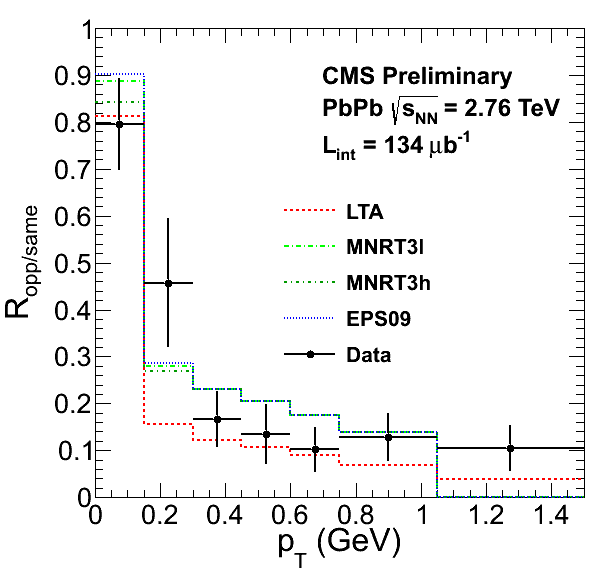
\includegraphics[angle=0,width=0.65\textwidth]{RoppSame.png}\\
%DIFDELCMD <                  %%%
%DIFDELCMD < \caption{%
{%DIFAUXCMD
\DIFdelFL{
        \label{fig:r4}  
         Ratio between the transverse momentum distribution of the J/$\psi$ when  J/$\psi$ and neutron have the opposite direction and the transverse momentum distribution of the J/$\psi$ when  J/$\psi$ and neutron have the same direction. 
            }}
           %DIFAUXCMD
\DIFdelendFL \DIFaddbeginFL 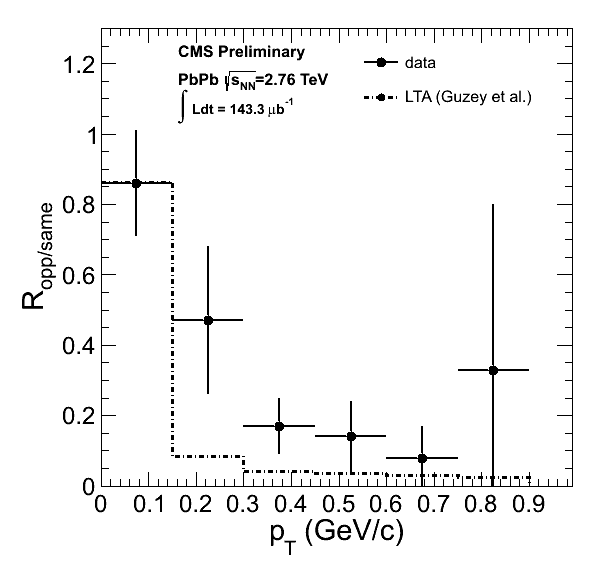
\includegraphics[angle=0,width=0.65\textwidth]{RoppsameVsTheory}
        \caption{\DIFaddFL{ \label{fig:r2} Ratio between the transverse momentum 
          distribution of the $J/\psi$ when  $J/\psi$ and neutron have 
          the opposite direction and the transverse momentum distribution 
          of the $J/\psi$ when  $J/\psi$ and neutron have the same direction.}}
      \DIFaddendFL \end{center}
    \end{figure*}
    \DIFdelbegin %DIFDELCMD < 

%DIFDELCMD <     %%%
\DIFdel{The rapidity distributions of the coherent and incoherent J/$\psi$ are shown in the Fig.~\ref{fig:r5}.  
    They are shown separately for the events firing the ZDC$^{+}$ and ZDC$^{-}$. 
    The same distributions are also obtained for the MC and shown in Fig.~\ref{fig:r6}.
      For the MC the particle gun generator with the input $p_{T}$ spectrum from 
      Zhalov's  calculation (LTA). 
    The rapidity symmetry for coherent J/$\psi$ and asymmetry for incoherent 
      J/$\psi$ are observed in data and MC.
  These are quantified in the Tab.~\ref{tab:uref}}\DIFdelend \DIFaddbegin \DIFadd{The same distributions as~\ref{fig:PtcorrandRation} but now as a function 
      of rapidity of the }\JPsi \DIFadd{are presented in the Fig~\ref{fig:r3} and 
      compiled in Fig.~\ref{fig:r4}}\DIFaddend . 

    \begin{figure*}[!Hhtb]
      \begin{center}
        \DIFdelbeginFL %DIFDELCMD < 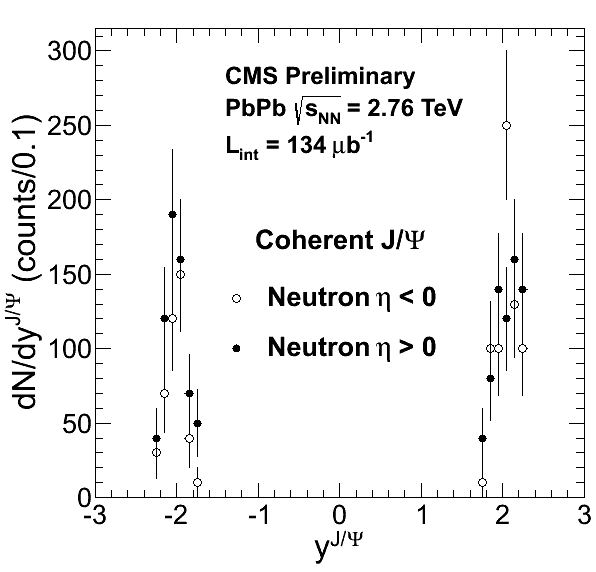
\includegraphics[angle=0,width=0.65\textwidth]{coherentRapidity1}%%%
\DIFdelendFL \DIFaddbeginFL 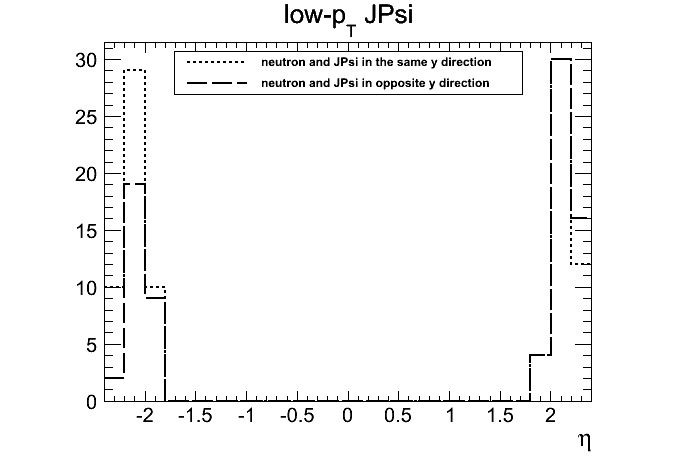
\includegraphics[angle=0,width=0.45\textwidth]{cohyOppAndSameNeutronDir}
        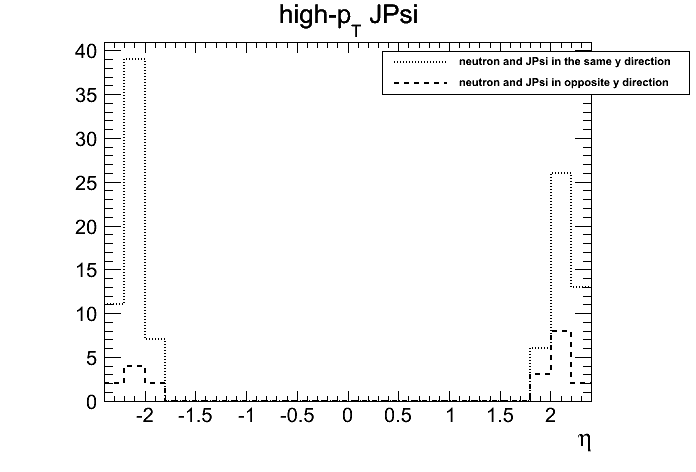
\includegraphics[angle=0,width=0.45\textwidth]{incohyOppAndSameNeutronDir}\DIFaddendFL \\
        \DIFdelbeginFL %DIFDELCMD < 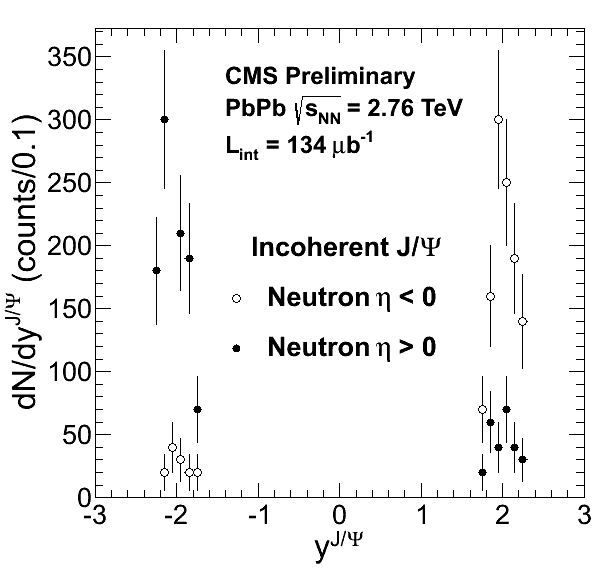
\includegraphics[angle=0,width=0.65\textwidth]{incoherentRapidity1}
%DIFDELCMD <              %%%
\DIFdelendFL \DIFaddbeginFL 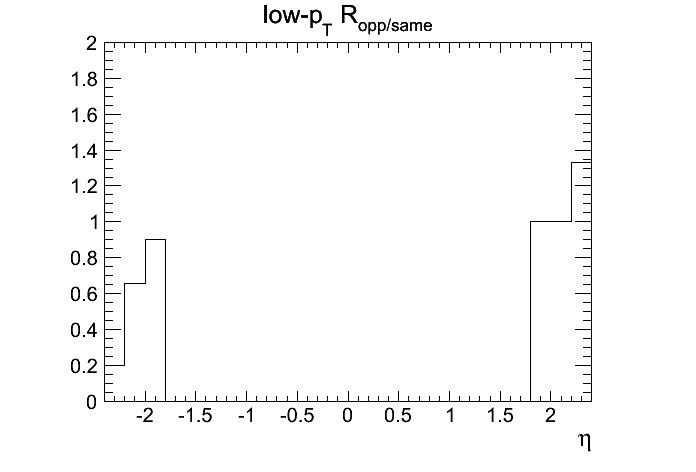
\includegraphics[angle=0,width=0.45\textwidth]{ratiocohyOppAndSameNeutronDir}
        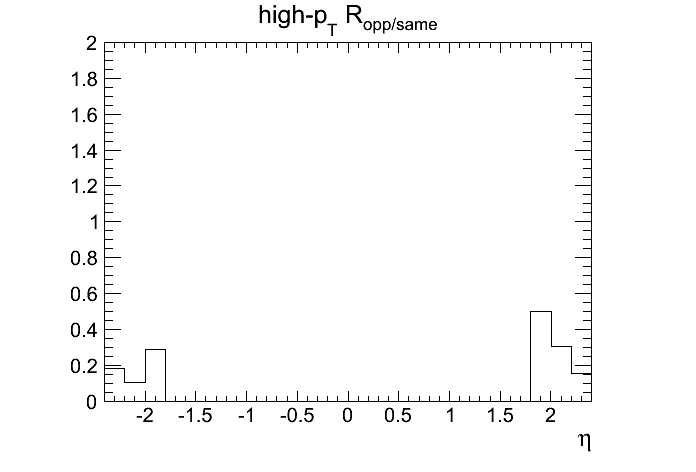
\includegraphics[angle=0,width=0.45\textwidth]{ratioincohyOppAndSameNeutronDir}
        \DIFaddendFL \caption{\DIFdelbeginFL \DIFdelFL{
        \label{fig:r5}  
        The }\DIFdelendFL \DIFaddbeginFL \DIFaddFL{ \label{fig:r3} Rapidity distribution of the $J/\psi$ when  
          $J/\psi$ and neutron have the opposite }\DIFaddendFL rapidity \DIFaddbeginFL \DIFaddFL{direction and the 
          rapidity }\DIFaddendFL distribution of the \DIFdelbeginFL \DIFdelFL{coherent }\DIFdelendFL \DIFaddbeginFL \DIFaddFL{$J/\psi$ when  $J/\psi$ and neutron 
          have the same rapidity direction for low-}\pt \DIFaddendFL (top \DIFaddbeginFL \DIFaddFL{left}\DIFaddendFL ) and \DIFdelbeginFL \DIFdelFL{incoherent }\DIFdelendFL \DIFaddbeginFL \DIFaddFL{high-}\pt 
          \DIFaddendFL (\DIFdelbeginFL \DIFdelFL{bottom}\DIFdelendFL \DIFaddbeginFL \DIFaddFL{top right}\DIFaddendFL ) \DIFdelbeginFL \DIFdelFL{J/$\psi$ }\DIFdelendFL \DIFaddbeginFL \JPsi\DIFaddFL{. Bottom: Ratios $R_{opp/same}$ }\DIFaddendFL for \DIFdelbeginFL \DIFdelFL{the  ZDC$^{+}$ }\DIFdelendFL \DIFaddbeginFL \DIFaddFL{low-}\pt \DIFaddFL{( left) 
          }\DIFaddendFL and \DIFdelbeginFL \DIFdelFL{ZDC$^{-}$}\DIFdelendFL \DIFaddbeginFL \DIFaddFL{high-}\pt \DIFaddFL{( right) }\JPsi\DIFaddendFL .}
      \end{center}
    \end{figure*}

    \begin{figure*}[!Hhtb]
      \begin{center}
        \DIFdelbeginFL %DIFDELCMD < 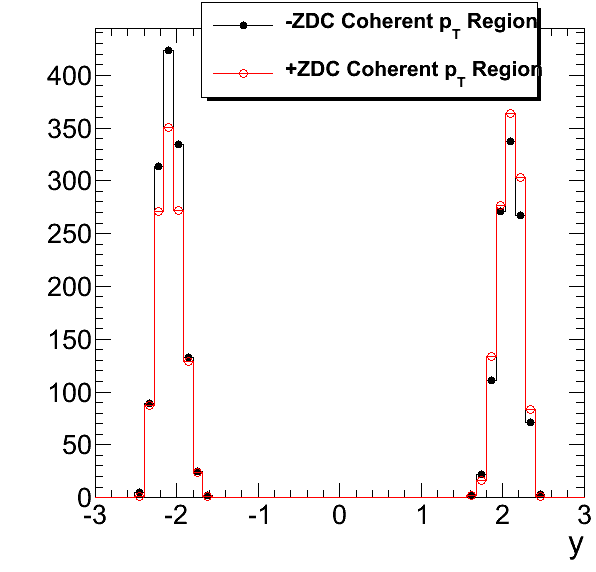
\includegraphics[angle=0,width=0.45\textwidth]{rapDistFromLTAGun.png}
%DIFDELCMD <             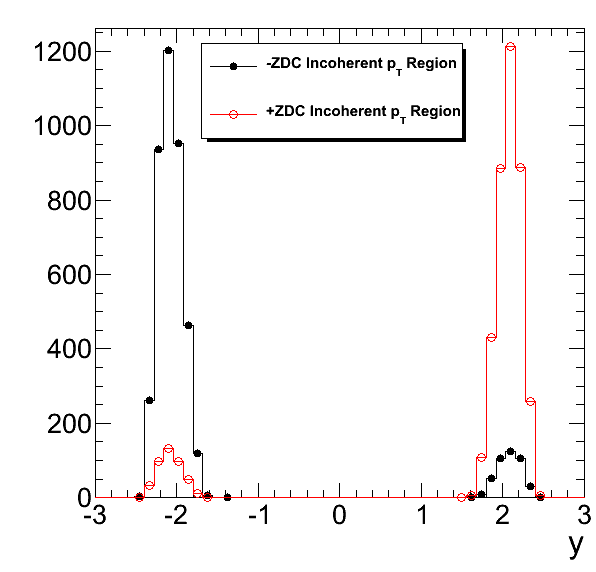
\includegraphics[angle=0,width=0.45\textwidth]{rapDistFromLTAGunInCo.png}
%DIFDELCMD <                  %%%
\DIFdelendFL \DIFaddbeginFL 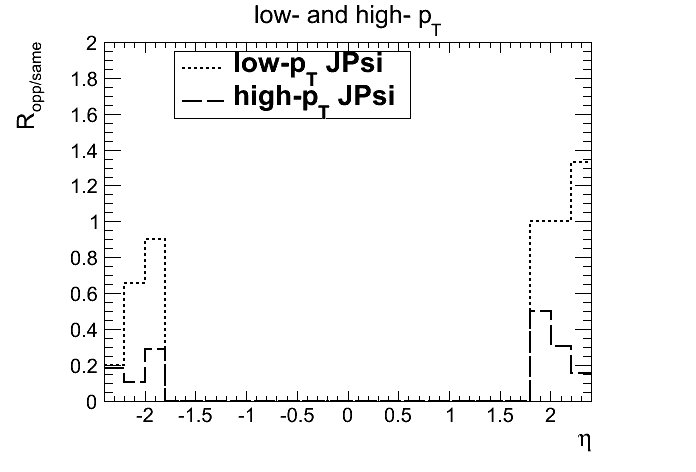
\includegraphics[angle=0,width=0.55\textwidth]{compiledratioincohandcohyOppAndSameNeutronDir}
        \DIFaddendFL \caption{\DIFdelbeginFL \DIFdelFL{
        \label{fig:r6}  
          The rapidity distribution of the coherent }\DIFdelendFL \DIFaddbeginFL \DIFaddFL{ \label{fig:r4} Rapidity ratios $R_{opp/same}$ for low-}\pt 
          \DIFaddendFL ( left) and \DIFdelbeginFL \DIFdelFL{incoherent }\DIFdelendFL \DIFaddbeginFL \DIFaddFL{high-}\pt \DIFaddendFL ( right) \DIFdelbeginFL \DIFdelFL{J/$\psi$ for the  ZDC$^{+}$ and ZDC$^{-}$ from MC (particle gun with customized $J/\psi p_{T}$ input distribution)}\DIFdelendFL \DIFaddbeginFL \JPsi\DIFaddendFL .}
      \end{center}
    \end{figure*}

    \DIFdelbegin \DIFdel{Table~\ref{tab:uref} gives the number of coherent and incoherent J/$\psi$ 
      separately }\DIFdelend \DIFaddbegin \DIFadd{Figure~\ref{fig:rNeutDimuCorr} shows the rapidity of the dimuon }\DIFaddend for the 
      events that \DIFdelbegin \DIFdel{fired the ZDC$^{-}$ and  ZDC$^{+}$. 
    We quote separately the J/$\psi$ that have the same or opposite rapidity direction to the neutron direction.The ratios, as described below are also given in the 
      Tab. 
    ~\ref{tab:uref}: 
      $R_{ZDC^{-}}^{y^{+}/y^{-}}$ : ratio between the number of J/$\psi$ having 
        }\DIFdelend \DIFaddbegin \DIFadd{are tagged by the ZDC$^{+}$ and  ZDC$^{-}$ means having 
      the neutron emitted in the }\DIFaddend $y>0$ \DIFdelbegin \DIFdel{to the 
      number of J/$\psi$ having }\DIFdelend \DIFaddbegin \DIFadd{and }\DIFaddend $y<0$\DIFdelbegin \DIFdel{from the events that fired 
        ZDC$^{-}$}\DIFdelend \DIFaddbegin \DIFadd{. 
    }

    \begin{figure*}[!Hhtb]
      \begin{center}
        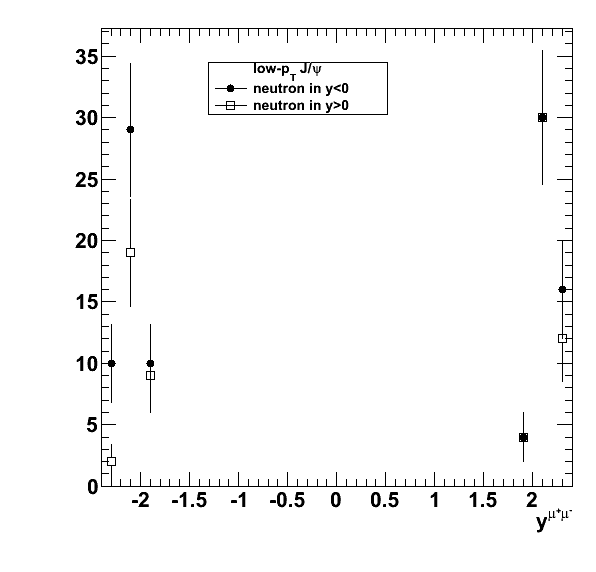
\includegraphics[angle=0,width=0.52\textwidth]{ZDCDimuCorrCoh}\DIFaddendFL \\
        \DIFdelbeginFL \DIFdelFL{$R_{ZDC^{+}}^{y^{-}/y^{+}}$ : ratio between the number of J/$\psi$ having 
        $y<0$ to the number of J/$\psi$ having $y>0$ from the events that fired 
        }\DIFdelendFL \DIFaddbeginFL 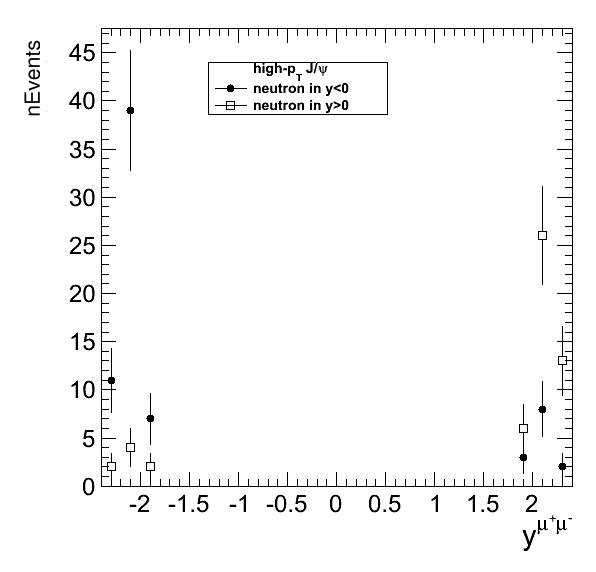
\includegraphics[angle=0,width=0.52\textwidth]{ZDCDimuCorrIncoh}\\
        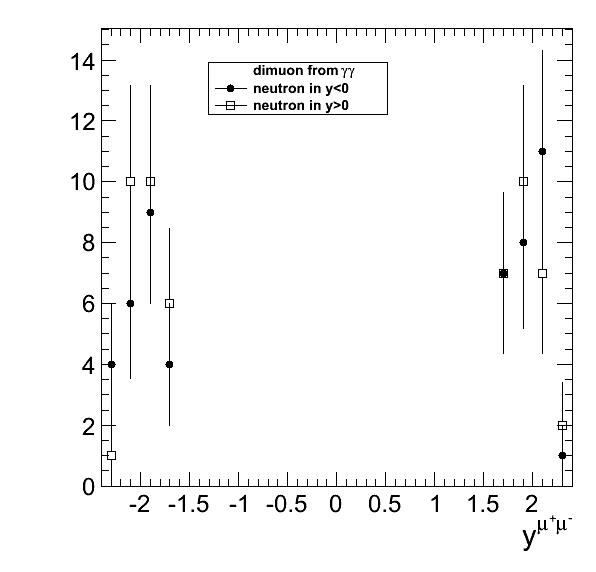
\includegraphics[angle=0,width=0.52\textwidth]{ZDCDimuCorrGammaGamma}
        \caption{\DIFaddFL{ \label{fig:rNeutDimuCorr} Rapidity distribution of }\JPsi \DIFaddFL{in the
          case of the events having the neutron in negative and positive rapidity 
          for the low-}\pt \JPsi \DIFaddFL{(top), high-}\pt \JPsi \DIFaddFL{(middle) and dimuons from
          $\gamma \gamma$ sample (bottom). }}
      \end{center}
    \end{figure*}

    \DIFadd{Another, interesting correlation between the }\JPsi \DIFadd{rapidity direction and 
      the neutron rapidity can be also studied with quantities defined in 
      Eq.~\ref{eq:Ration} that are calculated in the 
      Table~\ref{tab:corrneutronjpsi}. 
    Table~\ref{tab:corrneutronjpsieffcorr} gives the same quantities as  
      Table.~\ref{tab:corrneutronjpsi} but here it is corrected for the 
      difference between the efficiency of the }\DIFaddend ZDC$^{+}$ \DIFdelbegin %DIFDELCMD < \\
%DIFDELCMD <     %%%
\DIFdelend \DIFaddbegin \DIFadd{and  ZDC$^{-}$. 
    }\DIFaddend 

    \DIFaddbegin \begin{equation}\DIFadd{
      \label{eq:Ration}
      R_{(\mu\mu)^{-}}^{n^{-}/n^{+}} =  \frac{y^{-}_{\mu\mu} \wedge 
        y_{n}^{-}}{y^{-}_{\mu\mu} \wedge y_{n}^{+} }~~~~~~~~\mbox{and}~~~~~
        R_{(\mu\mu)^{+}}^{n^{-}/n^{+}} =  \frac{y^{+}_{\mu\mu} \wedge 
        y_{n}^{-}}{y^{+}_{\mu\mu} \wedge y_{n}^{+} }
    }\end{equation}

    \DIFaddend \begin{table}[h]
      \begin{center}
        \DIFdelbeginFL %DIFDELCMD < 

%DIFDELCMD <     %%%
%DIFDELCMD < \caption{%
{%DIFAUXCMD
\DIFdelFL{Final number of J/$\psi$ (for both ZDCs and for two negative and positive rapidity) and ratios with statistical uncertainty.}}
    %DIFAUXCMD
%DIFDELCMD < \label{tab:uref}
%DIFDELCMD <     %%%
\DIFdelendFL \begin{tabular}{|c|c|c|c|c|c|c|}
          \hline
          & \DIFdelbeginFL \DIFdelFL{ZDC$^{-}$ $y<0$ }\DIFdelendFL \DIFaddbeginFL \DIFaddFL{$y^{-}_{\mu\mu} \wedge y_{n}^{-}$ }\DIFaddendFL & \DIFdelbeginFL \DIFdelFL{ZDC$^{-}$ $y>0$ }\DIFdelendFL \DIFaddbeginFL \DIFaddFL{$y^{-}_{\mu\mu} \wedge y_{n}^{+}$ 
          }\DIFaddendFL & \DIFdelbeginFL \DIFdelFL{$R_{ZDC^{-}}^{y^{+}/y^{-}}$  }\DIFdelendFL \DIFaddbeginFL \DIFaddFL{$y^{+}_{\mu\mu} \wedge y_{n}^{+}$ }\DIFaddendFL & \DIFdelbeginFL \DIFdelFL{ZDC$^{+}$ $y<0$}\DIFdelendFL \DIFaddbeginFL \DIFaddFL{$y^{+}_{\mu\mu} \wedge y_{n}^{-}$ 
          }\DIFaddendFL & \DIFdelbeginFL \DIFdelFL{ZDC$^{+}$ $y>0$}\DIFdelendFL \DIFaddbeginFL \DIFaddFL{$R_{(\mu\mu)^{-}}^{n^{-}/n^{+}}$ 
          }\DIFaddendFL & \DIFdelbeginFL \DIFdelFL{$R_{ZDC^{+}}^{y^{-}/y^{+}}$ }\DIFdelendFL \DIFaddbeginFL \DIFaddFL{$R_{(\mu\mu)^{+}}^{n^{-}/n^{+}} $  }\DIFaddendFL \\ \hline
          \DIFdelbeginFL \DIFdelFL{coherent J/$\psi$ }\DIFdelendFL \DIFaddbeginFL \DIFaddFL{low-}\pt \JPsi \DIFaddendFL & \DIFdelbeginFL \DIFdelFL{63}\DIFdelendFL \DIFaddbeginFL \DIFaddFL{\textcolor{blue}{78 $\pm$ 8.8} 
          }\DIFaddendFL & \DIFdelbeginFL \DIFdelFL{68}\DIFdelendFL \DIFaddbeginFL \DIFaddFL{\textcolor{blue}{47 $\pm$  6.8}  }\DIFaddendFL & \DIFdelbeginFL \DIFdelFL{1.08$\pm$0.19}\DIFdelendFL \DIFaddbeginFL \DIFaddFL{\textcolor{blue}{81 $\pm$  9}  
          }\DIFaddendFL & \DIFdelbeginFL \DIFdelFL{42}\DIFdelendFL \DIFaddbeginFL \DIFaddFL{\textcolor{blue}{74 $\pm$  8.6} }\DIFaddendFL & \DIFdelbeginFL \DIFdelFL{69 }\DIFdelendFL \DIFaddbeginFL \DIFaddFL{\textcolor{blue}{ 1.66$\pm$0.31  } 
          }\DIFaddendFL & \DIFdelbeginFL \DIFdelFL{0.61$\pm$0.12 }\DIFdelendFL \DIFaddbeginFL \DIFaddFL{\textcolor{blue}{ 0.91$\pm$0.15  } }\DIFaddendFL \\ \hline
          \DIFdelbeginFL \DIFdelFL{incoherent J/$\psi$ }\DIFdelendFL \DIFaddbeginFL \DIFaddFL{high-}\pt \JPsi \DIFaddendFL & \DIFdelbeginFL \DIFdelFL{141 }\DIFdelendFL \DIFaddbeginFL \DIFaddFL{\textcolor{blue}{132 $\pm$  11.5}  
          }\DIFaddendFL & \DIFdelbeginFL \DIFdelFL{26}\DIFdelendFL \DIFaddbeginFL \DIFaddFL{\textcolor{blue}{17 $\pm$  4.1}  }\DIFaddendFL & \DIFdelbeginFL \DIFdelFL{0.184$\pm$0.039}\DIFdelendFL \DIFaddbeginFL \DIFaddFL{\textcolor{blue}{117 $\pm$  10.8}  
          }\DIFaddendFL & \DIFdelbeginFL \DIFdelFL{13}\DIFdelendFL \DIFaddbeginFL \DIFaddFL{\textcolor{blue}{29 $\pm$  5.4} }\DIFaddendFL & \DIFdelbeginFL \DIFdelFL{111}\DIFdelendFL \DIFaddbeginFL \DIFaddFL{\textcolor{blue}{7.76$\pm$2.0} 
          }\DIFaddendFL & \DIFdelbeginFL \DIFdelFL{0.117$\pm$0.034}\DIFdelendFL \DIFaddbeginFL \DIFaddFL{\textcolor{blue}{0.25$\pm$0.05 } }\DIFaddendFL \\ \hline
          \DIFaddbeginFL \DIFaddFL{$\mu^{+}\mu^{-}$ from $\gamma \gamma$ }& \DIFaddFL{\textcolor{blue}{80 $\pm$8.9} 
          }& \DIFaddFL{\textcolor{blue}{81 $\pm$9} }& \DIFaddFL{\textcolor{blue}{75 $\pm$8.7} 
          }& \DIFaddFL{\textcolor{blue}{83 $\pm$9.1} }& \DIFaddFL{\textcolor{blue}{0.99$\pm$0.16 } 
          }& \DIFaddFL{\textcolor{blue}{1.11$\pm$0.18} }\\ \hline
        \DIFaddendFL \end{tabular}
        \DIFaddbeginFL \caption{\label{tab:corrneutronjpsi} \DIFaddFL{Number of dimuon pairs for 
          different directions of the neutron rapidity direction together with 
          $R_{(\mu\mu)^{-}}^{n^{-}/n^{+}}$ and 
          $R_{(\mu\mu)^{+}}^{n^{-}/n^{+}}$.}}
      \DIFaddendFL \end{center}
    \DIFdelbeginFL %DIFDELCMD < 

%DIFDELCMD <     %%%
\DIFdelendFL \end{table}

    \DIFdelbegin \DIFdel{The combined ratio $R_{opp/same}^{c}$ is calculated as }\DIFdelend \DIFaddbegin \begin{table}[h]
      \begin{center}
        \begin{tabular}{|c|c|c|}
          \hline
          & \DIFaddFL{$R_{(\mu\mu)^{-}}^{\varepsilon_{ZDC}(n^{-}/n^{+})}$ 
          }& \DIFaddFL{$R_{(\mu\mu)^{+}}^{\varepsilon_{ZDC}(n^{-}/n^{+})} $  }\DIFaddendFL \\ \DIFdelbeginFL \begin{displaymath}\DIFdelFL{ R_{opp/same}^{c} = \frac{ZDC^{-} \mbox{and}~y>0 + ZDC^{+} 
      \mbox{and}~y<0}{ZDC^{-} \mbox{and}~y<0 + ZDC^{+} \mbox{and}~y>0} }\end{displaymath}%DIFAUXCMD
\DIFdelendFL \DIFaddbeginFL \hline
          \DIFaddFL{low-}\pt \JPsi &  \DIFaddFL{\textcolor{blue}{1.59 $\pm$ 0.29} 
          }& \DIFaddFL{\textcolor{blue}{0.88 $\pm$ 0.14} }\DIFaddendFL \\ \DIFdelbeginFL %DIFDELCMD < \begin{itemize}
%DIFDELCMD <       \item %%%
\DIFdelFL{$ R_{opp/same}^{c}$ for coherent J/$\psi$= 0.83 $\pm$ 0.12.
      }%DIFDELCMD < \item %%%
\DIFdelFL{$ R_{opp/same}^{c}$ for incoherent J/$\psi$= 0.155 $\pm$ 0.021.
    }%DIFDELCMD < \end{itemize}
%DIFDELCMD <     

%DIFDELCMD <     %%%
\DIFdelFL{The correction factors (efficiency, reconstruction) are as following: 
    }%DIFDELCMD < \begin{itemize}
%DIFDELCMD <       \item %%%
\DIFdelFL{$\epsilon_{ZDC^{-}}$: efficiency of the 
      ZDC$^{-}$ of 0.98
      }%DIFDELCMD < \item %%%
\DIFdelFL{$\epsilon_{ZDC^{+}}$: efficiency of the ZDC$^{+}$ of 0.94}%DIFDELCMD < \ 
%DIFDELCMD <       \item %%%
\DIFdelFL{$\epsilon_{\mu^{-}}$: efficiency $\times$ reconstruction of the muons 
        with rapidly $<$0: 1.0 
      }%DIFDELCMD < \item %%%
\DIFdelFL{$\epsilon_{\mu^{+}}$: efficiency $\times$ reconstruction of the muons 
        with rapidly $>$0: 1.014.
    }%DIFDELCMD < \end{itemize}
%DIFDELCMD <     

%DIFDELCMD <     %%%
\DIFdelFL{The combined ratio  $R_{opp/same}^{ceff}$ corrected with the factors  above is calculated as }\DIFdelendFL \DIFaddbeginFL \hline
          \DIFaddFL{high-}\pt \JPsi  & \DIFaddFL{\textcolor{blue}{7.45 $\pm$ 1.87}  
          }&  \DIFaddFL{\textcolor{blue}{0.24 $\pm$ 0.05 } }\DIFaddendFL \\ \DIFdelbeginFL \begin{displaymath}\DIFdelFL{ R_{opp/same}^{ceff} = \frac{\epsilon_{ZDC^{-}} \epsilon_{\mu^{+}} ZDC^{-} 
        \mbox{and}~y>0 + \epsilon_{ZDC^{+}} \epsilon_{\mu^{-}} ZDC^{+} 
        \mbox{and}~y<0}{\epsilon_{ZDC^{-}} \epsilon_{\mu^{-}} ZDC^{-} 
        \mbox{and}~y<0 + \epsilon_{ZDC^{+}} \epsilon_{\mu^{+}} ZDC^{+} 
        \mbox{and}~y>0} }\end{displaymath}
      %DIFAUXCMD
\DIFdelFL{$R_{opp/same}^{ceff}$ is 0.83$\pm$ 0.12. 
    }\DIFdelendFL \DIFaddbeginFL \hline
          \DIFaddFL{$\mu^{+}\mu^{-}$ from $\gamma \gamma$ 
          }& \DIFaddFL{\textcolor{blue}{0.95 $\pm$ 0.15} 
          }& \DIFaddFL{\textcolor{blue}{ 1.06 $\pm$ 0.17 } }\DIFaddendFL \\ \DIFaddbeginFL \hline
        \end{tabular}
        \caption{\label{tab:corrneutronjpsieffcorr} \DIFaddFL{Ratios 
          $R_{(\mu\mu)^{-}}^{\varepsilon_{ZDC}(n^{-}/n^{+})}$ and 
          $R_{(\mu\mu)^{+}}^{\varepsilon_{ZDC}(n^{-}/n^{+})} $ 
          i.e. $R_{(\mu\mu)^{-}}^{n^{-}/n^{+}}$ and 
          $R_{(\mu\mu)^{+}}^{n^{-}/n^{+}} $ corrected by the ZDC$^{+}$ and
          ZDC$^{-}$ efficiencies.}}
      \end{center}
    \end{table}
    \DIFaddend 

    \DIFdelbegin %DIFDELCMD < \begin{itemize}
%DIFDELCMD <       \item %%%
\DIFdel{$ R_{opp/same}^{ceff}$ for coherent J/$\psi$= 0.83 $\pm$ 0.12.
      }%DIFDELCMD < \item %%%
\DIFdel{$ R_{opp/same}^{ceff} $ for incoherent J/$\psi$= 0.154 $\pm$ 0.021.
    }%DIFDELCMD < \end{itemize}
%DIFDELCMD <     %%%
\DIFdelend \DIFaddbegin \DIFadd{Integrated over rapidity, separately for $y<0$ and $y>0$ ratios from 
      Table~\ref{tab:corrneutronjpsieffcorr} are shown in the 
      Figure~\ref{fig:integRatios}.
    }\DIFaddend 

    \DIFdelbegin \DIFdel{If considering 3 significant figures for the representation of the result these
      values are: 
    }%DIFDELCMD < \begin{itemize}
%DIFDELCMD <       \item %%%
\DIFdel{$ R_{opp/same}^{c}$ for coherent J/$\psi$= 0.833 $\pm$ 0.124
      }%DIFDELCMD < \item %%%
\DIFdel{$ R_{opp/same}^{c}$ for incoherent J/$\psi$= 0.155 $\pm$ 0.021
      }%DIFDELCMD < \item %%%
\DIFdel{$ R_{opp/same}^{ceff}$ for coherent J/$\psi$= 0.828 $\pm$ 0.124
      }%DIFDELCMD < \item %%%
\DIFdel{$ R_{opp/same}^{ceff} $ for incoherent J/$\psi$= 0.154 $\pm$ 0.021
    }%DIFDELCMD < \end{itemize}
%DIFDELCMD <     %%%
\DIFdelend \DIFaddbegin \begin{figure*}[!Hhtb]
      \begin{center}
        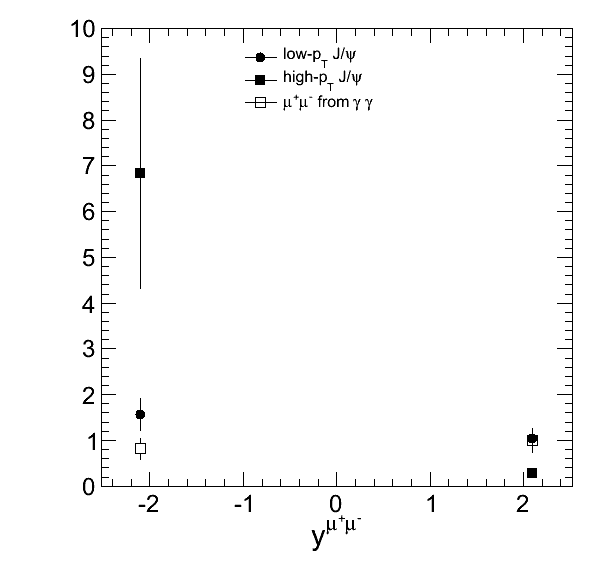
\includegraphics[angle=0,width=0.52\textwidth]{RCompiledYCorr}
        \caption{\DIFaddFL{ \label{fig:integRatios} 
          $R_{(\mu\mu)^{-}}^{\varepsilon_{ZDC}(n^{-}/n^{+})}$ and 
          $R_{(\mu\mu)^{+}}^{\varepsilon_{ZDC}(n^{-}/n^{+})}$ integrated over 
          one side in rapidity for low- and high-}\pt \JPsi \DIFaddFL{and also for dimuons
          from $\gamma \gamma$ sample. }}
      \end{center}
    \end{figure*}
    \DIFaddend 

    \DIFdelbegin \DIFdel{This shows that in this measurement the efficiencies factors are negligible}\DIFdelend \DIFaddbegin \DIFadd{From the Tab~\ref{tab:corrneutronjpsi} and the Fig.~\ref{fig:rNeutDimuCorr} 
      it is seen as expected that there is no correlation between the }\JPsi 
      \DIFadd{rapidity and neutron rapidity in the case of the low-}\pt \JPsi \DIFadd{and 
      dimuons coming from $\gamma \gamma$ sample. 
    In the case of the high-}\pt \JPsi \DIFadd{the correlation is clearly visible}\DIFaddend .  
